\documentclass[tikz,border=2pt]{standalone}
\usepackage{amsmath,amssymb}
\usepackage{tikz}
\usetikzlibrary{arrows.meta}

\begin{document}
% The feasible region is the intersection of all constraint half-planes: the shaded polygon.
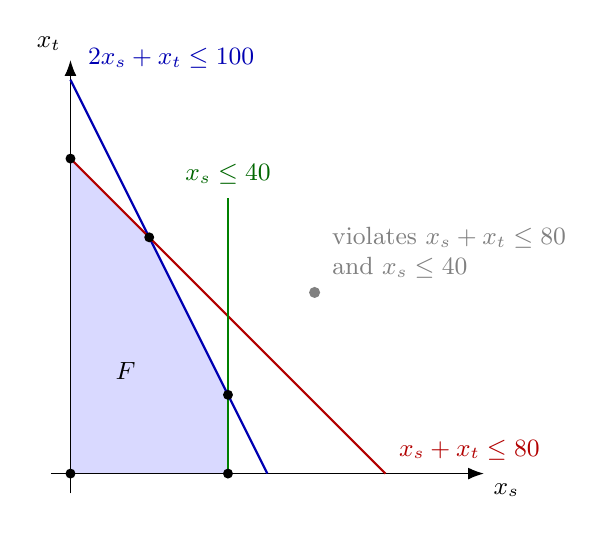
\begin{tikzpicture}[x=0.05cm, y=0.05cm, every node/.style={font=\small}, >={Latex[length=2mm]}]
	\fill[blue!15] (0,0) -- (40,0) -- (40,20) -- (20,60) -- (0,80) -- cycle;
	\draw[->] (-5,0) -- (105,0) node[below right] {$x_s$};
	\draw[->] (0,-5) -- (0,105) node[above left] {$x_t$};
	\draw[blue!70!black, thick] (50,0) -- (0,100);
	\draw[red!70!black, thick] (80,0) -- (0,80);
	\draw[green!50!black, thick] (40,0) -- (40,70);
	\foreach \p in {(0,0),(40,0),(40,20),(20,60),(0,80)} {\fill[black] \p circle (1.8pt);}
	\node[blue!70!black, font=\small, anchor=south west] at (2,100.5) {$2x_s+x_t\le100$};
	\node[red!70!black, font=\small, anchor=south west] at (81,1) {$x_s+x_t\le80$};
	\node[green!40!black, font=\small, anchor=south] at (40,71) {$x_s\le40$};
	\node[font=\small] at (14,26) {$F$};
	\fill[gray] (62,46) circle (2pt);
	\node[gray, font=\small, anchor=south west, align=left] at (64,47) {violates $x_s+x_t\le80$\\ and $x_s\le40$};
	\end{tikzpicture}
\end{document}
